%!TEX root = ../../Master.tex
\section{Graph theory}

Graph theory is frequently used in computer science to model some kind of relationship between objects. These objects could be anything. Graph theory is a preferred method to model building complexes, because it can precisely model how e.g. a hallway in a hospital is connected to a room.

In graph theory objects are called \enquote{nodes} or \enquote{vertices}. The two terms can be used interchangeably. In this report, vertices will describe locations or POI (points of interest) in a hospital. Another term in graph theory is an edge. This is basically connecting two vertices and thereby providing a relationship between these vertices. See \cref{fig:labeled_graph}. An edge can be seen as a possible route connecting one location to another. Now in order to describe the relationship between two vertices, we use an weighted graph in which an edge has a number attribute called a weight. A weight can describe the time, distance or any other metric that in some way can describe how two connected vertices are related\cite{wiki_graph_glos,MIT2012}.

We can describe these definitions formally.\cite{MIT2012}
\begin{mydef}
	A graph $G$ is a pair of sets $(V,E)$ where $V$ is a non-empty set of items called vertices or nodes. $E$ is a set of 2-item subsets of $V$ called edges.
\end{mydef}

\begin{figure}[ht!]
    \centering
    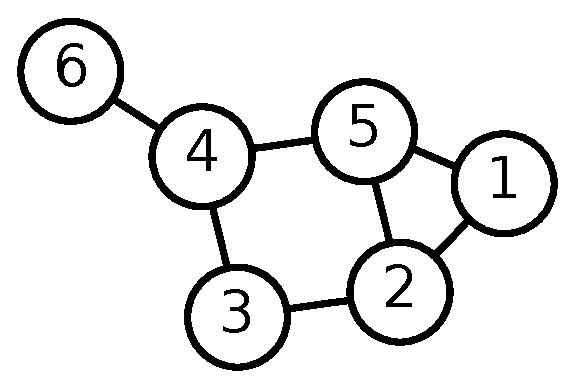
\includegraphics[width=0.5\textwidth]{6n-graf.eps}
    \caption{A labeled simple graph with vertex set $V = \left\{ {1, 2, 3, 4, 5, 6} \right\} $ and edge set $E = \left\{ \left\{ {1,2}\right\}, \left\{ {1,5}\right\}, \left\{ {2,3}\right\}, \left\{ {2,5}\right\}, \left\{ {3,4}\right\}, \left\{ {4,5} \right\} , \left\{ {4,6} \right\} \right\}$. \cite{wiki_graph_glos}}
    \label{fig:labeled_graph}
  \end{figure}

%!TEX root = ../../Master.tex
\subsection{Directed and Undirected Graphs}

\cref{fig:labeled_Directed_undirected} shows two graphs, one is directed and the other is undirected. Graph 1 is undirected and does not have a specific direction. Graph 2 is directed which means the edges is one way only. The arrows indicates the direction the edges allow. This means vertex 1 can go to vertex 2 and 3, but neither can go back. 


\begin{figure}[ht!]
    \centering
    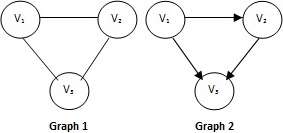
\includegraphics[width=0.5\textwidth]{Directed_undirected.png}
    
    \caption{Graph 1 is directed and graph 2 is undirected. From \cite{dir_pic}}\label{fig:labeled_Directed_undirected}


  \end{figure}

\subsection{Representation of graphs}

Two standard ways to represent a graph exists: as a collection of adjacency lists or as an adjacency matrix. Both representations support directed and undirected graphs. Each representation method has its merits \cite{Cormen2009}.

\subsubsection{Adjacency list}
Adjacency lists provide a very compact way to represent \textbf{sparse} graphs. The keyword is sparse. Adjacency lists are only compact and the preferred representation of graphs if the number of edges in a graph is much less than the number of vertices squared. \cref{fig:labeled_graph,fig:labeled_Directed_undirected} are represented as a collection of adjacency lists.

\subsubsection{Adjacency matrix}
Adjacency matrices are usually the representation of choice when the graph is \textbf{dense}. This means that adjacency matrices should be used when the number of edges is close to the number of vertices squared. Adjacency matrices also has the merit of providing quick lookup of which vertices are connected. See \cref{fig:adjacency_matrix} for an example.

\begin{figure}[ht!]
    \centering
    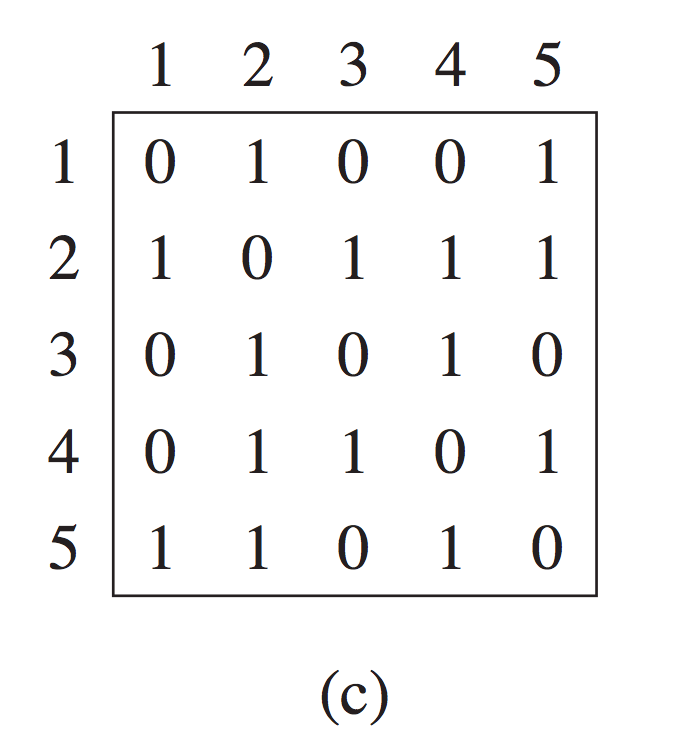
\includegraphics[width=0.5\textwidth]{adjacency_matrix}
    \caption{An example of an adjacency matrix. Row and column numbers are vertex ids. The content of the matrix is the weight the connection between row vertex and column vertex has \cite{Cormen2009}}.
    \label{fig:adjacency_matrix}
  \end{figure}


